\vspace{-3mm}
\section{Introduction}
\label{sec:introduction_011}

\looseness=-1
An agent is expected to satisfy three important properties for a reliable deployment in real-world applications: \textbf{(i)} The agent should learn \emph{fast} with as few episode failures as possible. \textbf{(ii)} The agent should \emph{maintain high reward} when facing new environments similar to the training environment after deployment. \textbf{(iii)} The agent should \emph{flag anomalous environment states} when it does not know what action to take in an unknown environment. These three practically desirable properties translate into three technical properties in reinforcement learning agents. Indeed, a reinforcement learning agent should achieve high \emph{sample efficiency} at training time \cite{sample-efficient-ac}, high \emph{generalization} performance on test environments similar to the training environment \cite{epistemic-pomdp}, and high \emph{Out-Of-Distribution (OOD) detection} scores on environment unrelated to the training task \cite{ood-detection-survey, ood-automotive-perception}. 

\looseness=-1
In this paper, we argue that \emph{aleatoric} and \emph{epistemic} uncertainty are key concepts to achieve these desired practical and technical properties. The aleatoric uncertainty represents the irreducible and inherent stochasticity of the environment. Thus, an environment region with high aleatoric uncertainty is unlikely to be interesting to explore at training time because it could be uninformative (e.g. a sensor is very noisy) or dangerous (e.g. the environment has an unpredictable behavior). In contrast, the epistemic uncertainty represents the lack of information for accurate prediction. Thus, an environment region with high epistemic uncertainty is potentially promising to explore to build a better understanding of the environment (e.g., a state has unknown transition dynamics because it has never been explored).

\begin{figure}[t]
    \centering
    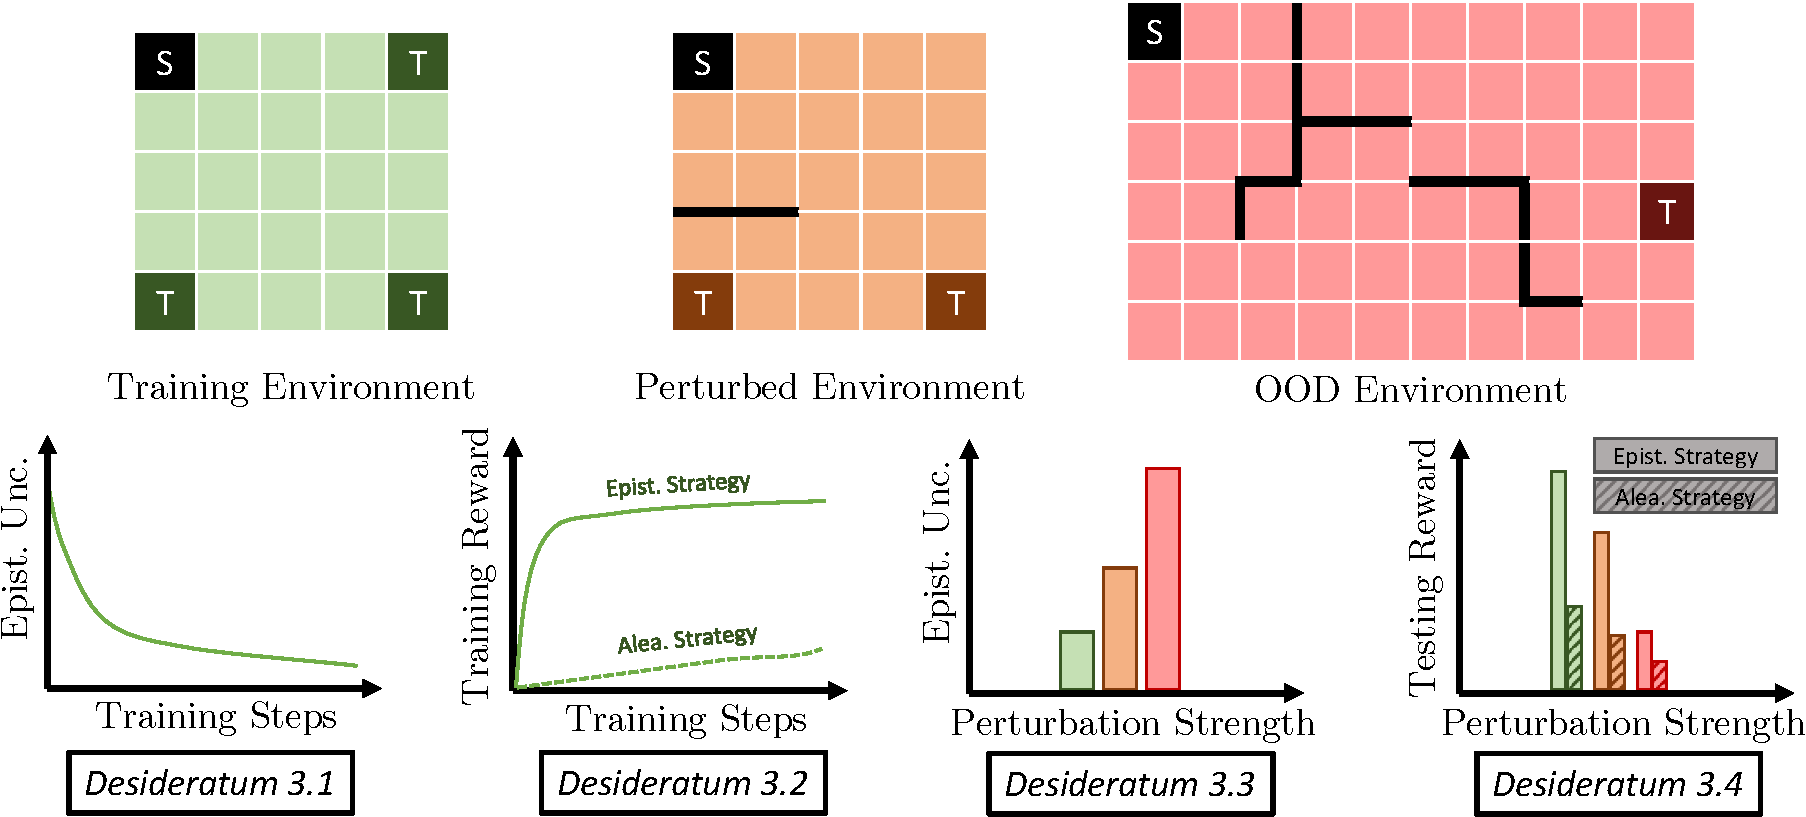
\includegraphics[width=.99\linewidth]{sections/011_icml2022/resources/diagram-cropped_2.pdf}
    \caption{Overview of our proposed desiderata for uncertainty in RL (See sec.~\ref{sec:desiderata_011}).}
    \label{fig:diagram}
\end{figure}

\looseness=-1
The core motivation of our work is to disentangle the properties of aleatoric and epistemic uncertainty estimates in RL to build agents with reliable performance in real-world applications. This motivation is similar to supervised learning (SL) where previous works defined \emph{desiderata}, \emph{models}, and \emph{evaluation} methods for aleatoric and epistemic uncertainty \cite{uncertainty-deep-learning, review-uncertainty-dl, dataset-shift, robustness-uncertainty-dirichlet}. Important examples of models using a single or multiple forward passes for uncertainty estimation in SL are MC dropout \cite{dropout}, ensemble \cite{ensembles, hyper-ensembles, batch-ensembles}, deep kernel learning \cite{simple-baseline-uncertainty, due, duq, uceloss}, and evidential networks \cite{postnet, priornet, natpn, evidential-regression}. Further, empirical evaluation of uncertainty estimates in SL focuses \emph{only} on testing time with Out-Of-Distribution (OOD) detection and generalization or detection of shifts \citep{dataset-shift, shifts-dataset}. In contrast to SL, the RL setting is more complex since it cares about the performance of uncertainty estimates at \emph{both} training and testing time.

\looseness=-1
\textbf{Our Contributions.} In this work, we propose a framework for aleatoric and epistemic uncertainty estimation in RL: \textbf{(Desiderata)} We explicitly define four desiderata for uncertainty estimation in RL at both \emph{training} and \emph{testing time} (See fig.~\ref{fig:diagram}). They cover the behavior of \emph{aleatoric} and \emph{epistemic} uncertainty estimates w.r.t. the sample efficiency in the training environment and, w.r.t. the generalization performance in different testing environments. \textbf{(Models)} We carefully combine a diverse set of uncertainty estimation methods in SL (i.e. MC dropout, ensemble, deep kernel learning, and evidential networks) with Deep Q-Networks (DQN) \cite{dqn}, an ubiquitous RL model that is not equipped with uncertainty estimate by default. These combinations require a \emph{minimal} modification to the training procedure of the RL agent. We discuss \emph{theoretical} evidence on the ability of these combinations to fulfill the uncertainty desiderata. \textbf{(Evaluation)} Finally, we also propose a \emph{practical} methodology to evaluate uncertainty in RL based on OOD environments and domain shifts.
